\chapter{Analysis and Specification of Needs}

\section{Introduction}

In this chapter, we will present the analysis and specification of needs. We start by presenting the specification of the requirements, illustrating them using the diagram of the global use cases. Then we will present our project architecture and our working environment, and finally we will present our product backlog and releases planning, and we will close our chapter with a conclusion.

\section{Requirements Specification}

In this section, we will define the actors of our application and the functional and non-functional needs that our application aims to fulfill.

\subsection{Identifying Actors}

We define actors as a shorthand for the roles played by entities outside the system that interact directly with them. In our system, we identify four types of actors:

\begin{itemize}
    \item \textbf{\textcolor{primary}{Super Admin}}: Responsible for the global configuration of the platform, they have extended privileges to manage administrators, oversee security, and ensure compliance. They can also configure advanced features and control all system resources.
    
    \item \textbf{\textcolor{primary}{Admin}}: In charge of the day-to-day management of the platform, they can add, modify, or delete listings, supervise agency and user profiles, and ensure smooth operations. They are also responsible for monitoring and assisting other actors.
    
    \item \textbf{\textcolor{primary}{Real Estate Agent}}: Dedicated to creating and updating real estate listings, they manage property information, handle investor requests, and finalize transactions related to sales or rentals. They can also coordinate property visits and propose tailored offers.
    
    \item \textbf{\textcolor{primary}{Investor}}: A user who wishes to browse and finance real estate projects. They have access to all available offers, can make investments in a few simple steps, and monitor the evolution of their portfolio. They also benefit from personalized insights to optimize their investments.
    
    \item \textbf{\textcolor{primary}{System}}: The entity that automatically manages all basic functionalities, such as authentication, notification generation, transaction validation, and adherence to security protocols. It ensures the coherence and reliability of the application at all times.
\end{itemize} 

\subsection{Functional Requirements}

After several meetings with our client, the various functional requirements of our application are illustrated as follows:

\subsubsection{For the Super Admin (Korpor)}
\begin{itemize}
    \item \textbf{Authenticate}: The super admin enters their credentials to access the advanced management console.
    \item \textbf{Log Out}: After viewing or updating global settings, they can securely log out.
    \item \textbf{Manage Admin Accounts}: Create, enable/disable, or modify admin profiles associated with different real estate companies.
    \item \textbf{Monitor Security \& Compliance}: Oversee transactions, data integrity, and regulatory adherence using specialized reporting and audit tools.
    \item \textbf{Configure Platform Features}: Define key parameters (payment methods, AI/blockchain integrations, etc.) and roll out feature updates.
    \item \textbf{View Global Reports}: Generate and analyze consolidated metrics (financials, user activity, transactions) for overall performance insights.
    \item \textbf{Moderate Content}: Review and remove any inappropriate or erroneous property listings or user-generated data.
\end{itemize} 

\subsubsection{For the Admin (Real Estate Company)}
\begin{itemize}
    \item \textbf{Authenticate}: The admin logs in with valid credentials to manage daily operations.
    \item \textbf{Log Out}: They can end their session to maintain account security.
    \item \textbf{Manage Real Estate Listings}: Add, update, or delete property listings visible to investors.
    \item \textbf{Oversee Real Estate Agents}: Create and manage agent accounts, assign properties, and monitor performance and commissions.
    \item \textbf{Track Transactions \& Commissions}: Review incoming payments, calculate commissions owed to agents, and track the history of completed deals.
    \item \textbf{Address Investor Inquiries}: Respond to questions or concerns from investors, ensuring a smooth user experience.
    \item \textbf{Access Agency Dashboard}: View comprehensive statistics on properties, sales, rentals, and market trends.
\end{itemize}

\subsubsection{For the Real Estate Agent}
\begin{itemize}
    \item \textbf{Authenticate}: The agent logs in to manage assigned properties and interact with potential investors.
    \item \textbf{Log Out}: Securely exit the account after completing tasks.
    \item \textbf{Manage Assigned Properties}: Create new listings, update property details, set prices, and upload images.
    \item \textbf{Handle Investment Requests}: Review purchase or rental offers, negotiate terms, and initiate contract finalization.
    \item \textbf{Contribute to AI Estimates}: Provide or refine data to improve AI-driven pricing and market analysis.
    \item \textbf{Maintain Client Relationships}: Communicate with investors, schedule property visits, and follow up on inquiries.
    \item \textbf{View Commissions}: Track earnings based on successful sales or rentals.
\end{itemize}

\subsubsection{For the Investor (Mobile App User)}
\begin{itemize}
    \item \textbf{Create an account \& authenticate}: Register to gain access to the platform's core features.
    \item \textbf{Log Out}: End the session to protect personal and financial data.
    \item \textbf{Browse Listings \& Invest}: Explore available properties, filter according to preferences, and commit to an investment in a few steps.
    \item \textbf{Track Portfolio}: Monitor owned assets, property status, and receive real-time updates on performance.
    \item \textbf{Make Payments}: Use integrated payment methods (credit cards, digital wallets, etc.) to complete transactions.
    \item \textbf{Access AI Recommendations}: View data-driven insights and return-on-investment estimates generated by the system.
    \item \textbf{Manage Withdrawals \& Earnings}: Withdraw profits, monitor rental income, or exit investments under the right conditions.
\end{itemize}

\subsubsection{For the System}
\begin{itemize}
    \item \textbf{Automate Authentication}: Validate credentials, manage sessions, and maintain user roles and permissions.
    \item \textbf{Generate Notifications}: Send real-time alerts (e.g., new listings, completed transactions, commission updates) to relevant users.
    \item \textbf{Ensure Compliance \& Security}: Leverage blockchain for data integrity, verify payments, and detect anomalies or fraudulent activities.
    \item \textbf{Coordinate AI Insights}: Aggregate and analyze real estate data to produce market predictions and price recommendations.
    \item \textbf{Maintain Transaction Consistency}: Update dashboards, user balances, and property statuses automatically upon each operation.
    \item \textbf{Optimize Performance}: Monitor server load, scale resources, and ensure a smooth, responsive application experience.
\end{itemize} 

\subsection{Non-functional Requirements}

In order to ensure the proper functioning of the decision-making system and to avoid any kind of anomaly, the implemented solution must meet a set of non-functional needs such as:

\begin{itemize}
    \item \textbf{Maintainability}: The system must be designed for simplicity so that tasks, updates, and bug fixes can be executed with minimal complexity.
    
    \item \textbf{Evolution}: Platform administration must remain attentive to user needs and feedback, continuously enhancing the services offered while preserving the application's utility and efficiency.
    
    \item \textbf{Security}: Robust security measures are essential. The platform must enforce strong authentication protocols, access privileges, and comprehensive data encryption (both at rest and in transit). The integration of blockchain technology further ensures the immutability and integrity of sensitive information.
    
    \item \textbf{Efficiency}: The application must be effective in all circumstances, delivering prompt and reliable functionality regardless of external conditions.
    
    \item \textbf{Performance}: The system must operate optimally across diverse environments. It should consistently provide a responsive and reliable experience, even under high transaction volumes or varying network conditions.
\end{itemize} 

\section{Requirements Analysis}

In this section, we'll outline the various features that our app should offer, using a general use case diagram.

\subsection{General use case diagram}

Below, we present the various actors of the application and the actions they are authorized to perform.
The overall diagram is illustrated in the following figure:

\begin{figure}[htbp]
    \centering
    % Replace with actual image file once available
    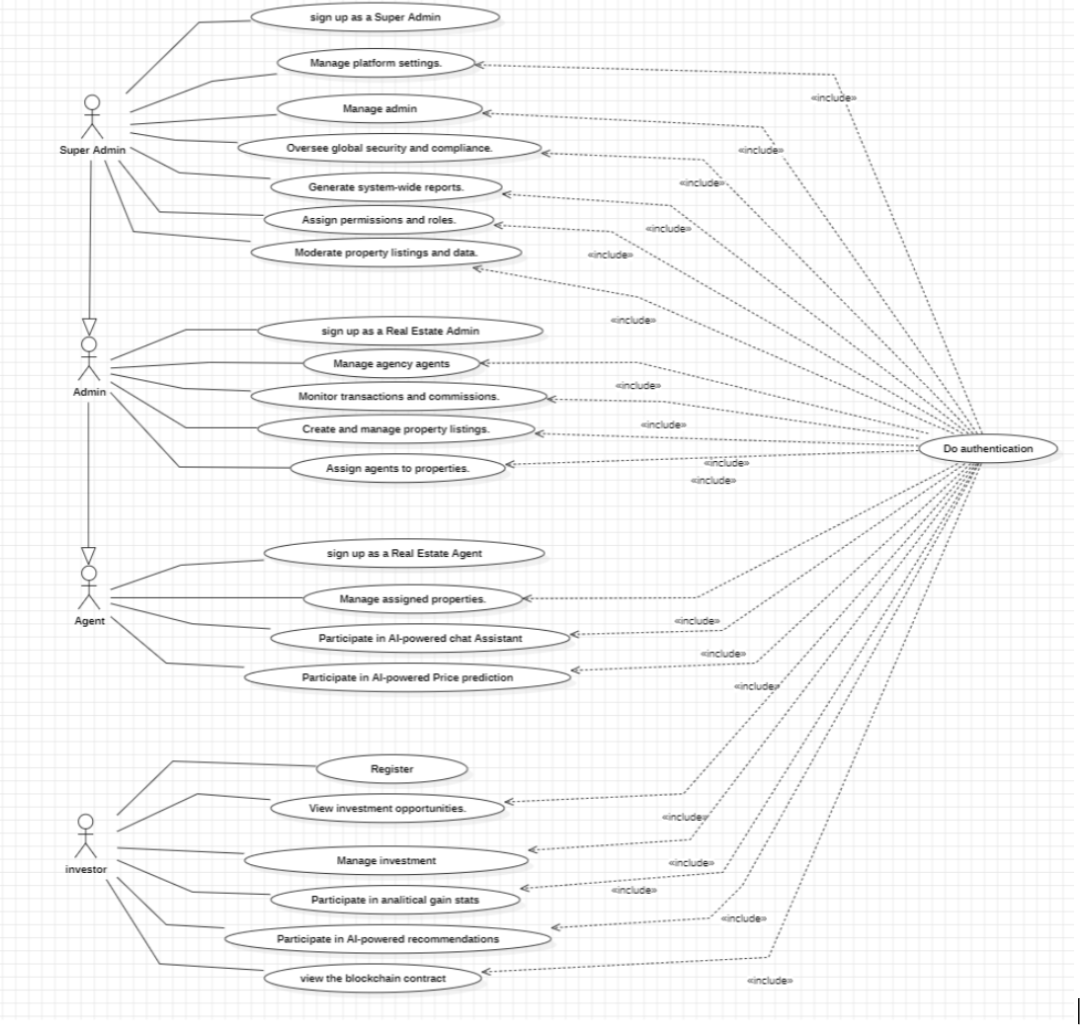
\includegraphics[width=0.85\textwidth]{images/diagram de case d utilisation general.png}
    \caption{General use case diagram}
    \label{fig:use-case-diagram}
\end{figure}